\documentclass[twoside]{report}
\usepackage[italian]{babel}
\usepackage[utf8]{inputenc}
\usepackage{amsmath}
\usepackage{amsthm}
\usepackage{amsfonts}
\usepackage{amssymb}
\usepackage{cancel}
\usepackage[margin=1in]{geometry}
\usepackage{hyperref}
\usepackage{bookmark}
\usepackage{setspace}
\usepackage{titlesec}
\usepackage{fancyhdr}
\usepackage{adjustbox}
\usepackage{float}
\usepackage{listings}
\usepackage{graphicx}

\graphicspath{{./images/}}

\setlength{\parskip}{0pt}
\titlespacing*{\subparagraph}{1em}{0em}{0em} 

\makeatletter
\renewenvironment{abstract}{%
    \if@twocolumn
        \section*{\abstractname}%
    \else
        \begin{center}%
            {\bfseries \abstractname\vspace{-.5em}\vspace{\z@}}%
        \end{center}%
        \small
        \begin{quotation}
    \fi}
    {\if@twocolumn\else\end{quotation}\fi}
\makeatother

\hypersetup{
    pdfauthor={Luca Facchini},
    pdftitle={Appunti di Basi di Dati},
    pdfsubject={Appunti del corso di Basi di Dati tenuto dal prof. Bouquet Paolo presso l'Università degli Studi di Trento nell'anno accademico 2024/2025},
    pdfkeywords={Reti, Università degli Studi di Trento, Bouquet Paolo, Luca Facchini},
    pdfproducer={LaTeX},
    pdfcreator={pdflatex},
}

\fancypagestyle{chapterInit}{
    \pagestyle{stdPage}
    \fancyhead{}
    \renewcommand{\headrulewidth}{0pt}
}

\fancypagestyle{stdPage}{
    \renewcommand{\footrulewidth}{0.4pt}
    \fancyhead{}
    \fancyhead[RO,LE]{\leftmark}
    \fancyhead[RE,LO]{\rightmark}
    \fancyfoot{}
    \fancyfoot[LE,RO]{\thepage}
    \fancyfoot[LO,RE]{"Appunti di Basi di Dati" di Luca Facchini}
}

\def\ojoin{\setbox0=\hbox{$\bowtie$}%
  \rule[-.02ex]{.25em}{.4pt}\llap{\rule[\ht0]{.25em}{.4pt}}}
\def\leftouterjoin{\mathbin{\ojoin\mkern-5.8mu\bowtie}}
\def\rightouterjoin{\mathbin{\bowtie\mkern-5.8mu\ojoin}}
\def\fullouterjoin{\mathbin{\ojoin\mkern-5.8mu\bowtie\mkern-5.8mu\ojoin}}

\newcommand{\<}{\textless}
\renewcommand{\>}{\textgreater}

\title{Appunti di Basi di Dati}
\author{Luca Facchini (mat. 245965)}
\date{A.A. 2024/2025}

\begin{document}
    \begin{titlepage}
        \centering  % Center everything on the title page
        {\Huge\textbf{Appunti di Basi di Dati}} \\[1cm] % Title
        \vspace{0.5cm}
        
        {\Large Luca Facchini} \\ % Author name
        \vspace{0.3cm}
        {\large Matricola: 245965} \\[2cm] % Additional author info
        
        {\large Corso tenuto dal prof. Bouquet Paolo} \\[0.3cm] % Course information
        {\large Università degli Studi di Trento} \\[1.5cm]
        
        {\large A.A. 2024/2025} \\[3cm] % Academic year
        
        % Abstract section with spacing control
        \vfill
        \begin{abstract}
            Questo documento contiene gli appunti del corso di Basi di Dati tenuto dal prof. Bouquet Paolo presso l'Università degli Studi di Trento nell'anno accademico 2024/2025.
        \end{abstract}
        
        \vfill  % Pushes the content to the center vertically
    \end{titlepage}
    \tableofcontents

    \pagestyle{stdPage}
    

    \chapter{Il Modello Relazionale}
\label{cap:il-modello-relazionale}
\thispagestyle{chapterInit}

\section{Concetti Generali}
    \paragraph{La Storia} Il modello fu proposto da Edgar F. Codd nel 1970 nel suo articolo: "A Relational Model of Data for Large Shared Data Banks".
    \paragraph{Il Modello} Il modello relazionale è un modello di dati che si basa sul concetto matematico di relazione.
\section{Relazione} 
    \paragraph{Definizione}
        \textit{Informalmente}, una \textbf{relazione} può essere vista come una \textbf{tabella} con un insieme di valori su ogni riga. 
        
        Ci sono due livelli che definiscono una relazione:
        \begin{itemize}
            \item Lo \textbf{schema} della relazione (livello \textit{intensionale})
            \item \textbf{Istanze} della relazione (livello \textit{estensionale})  
        \end{itemize}
    \subsection{Definizione intensionale} Lo schema di una   relazione definisce:
            \begin{itemize}
                \item Il nome della relazione
                \item il nome di ogni attributo
                \item il dominio di ogni attributo
            \end{itemize}
            Si nota come l'ordine degli attributi non sia rilevante. Uno dei modi "standard" di rappresentare una relazione è il seguente: \texttt{Students(\textit{sid}: string, \textit{name}: string, \textit{login}: string, \textit{age}: integer, \textit{gpa}: real)}.
            \paragraph{Grado} Il \textbf{grado} di una relazione è il numero di attributi che la compongono (nel caso dell'esempio, il grado è 5).
    \subsection{Definizione estensionale} Un'istanza di uno schema di relazione è un \underline{insieme} di \textbf{tuple} (o \textbf{record}), ognuna delle quali ha lo stesso numero di campi dello schema della relazione. Questo comporta:
        \begin{itemize}
            \item Essendo un insieme \textbf{non} possono esserci duplicati
            \item L'ordine delle tuple non è rilevante
        \end{itemize}
        \paragraph{Cardinalità} La \textbf{cardinalità} di una relazione è il numero di tuple che contiene.
    \subsection{Stato di una relazione}
        Lo \textbf{stato di una relazione} è un sottoinsieme del prodotto cartesiano dei domini dei suoi attributi:
        
        Data una relazione: $ R(A_1, A_2, \dots, A_n) $, lo stato di $ R $ è definito come: 
        $$
            r(R)\subset \operatorname{dom}(A_1)\times \operatorname{dom}(A_2)\times \dots \times \operatorname{dom}(A_n)
        $$
        ovvero:
        $$
            \begin{aligned}
                r(R)&= \{t_1, t_2, \dots, t_n\}\qquad & \text{dove ogni } t_i \text{ è una tupla}\\
                t_i&= \left< v_1, v_2, \dots, v_n \right> \qquad & \text{dove } v_i \text{ è un elemento dell'attributo } \operatorname{dom}(A_j)
            \end{aligned}
        $$
    \subsection{Chiave di una relazione}
        Ogni riga di una relazione ha un campo (o un insieme di campi) il cui valore (o i cui valori) identifica univocamente quella la riga in quella tabella. Questo campo (o insieme di campi) è detto \textbf{chiave} della relazione.

        Talvolta si usano valori convenzionali per identificare una riga in una tabella. Si parla di \textit{chiave artificiale} (\textit{artificial key}) o \textit{chiavi surrogate} (\textit{surrogate key}).
\section{Vincoli}
    \paragraph{Definzione} I vincoli determinano quali stati di una relazione in una base di dati relazionale sono ammissibili e quali non lo sono.
    
    Esistono tre tipi di vincoli:
    \begin{enumerate}
        \item \textbf{Vincoli Impliciti:} dipendono dal \textit{data model} stesso.
        \item \textbf{Vincoli basati sullo schema } ( o \textbf{espliciti}): sono definiti nello schema usando gli strumenti forniti dal modello \textbf{ER}.
        \item \textbf{Vincoli applicativi o semantici:} si trattano di vincoli che vanno al di là del modello e devono essere imposti a livello di programma
    \end{enumerate}
    Un vincolo è definito come una \textbf{condizione} che DEVE valere affinché lo \textbf{stato} di una relazione sia \textbf{valido}. 

    I principali tipi di vincoli espliciti che possono essere espressi nel modello relazionale sono:
    \begin{itemize}
        \item Vincolo di \textbf{dominio}
        \item Vincolo di \textbf{chiave}
        \item Vincolo di \textbf{integrità} delle \textbf{entità}
        \item Vincolo di \textbf{integrità referenziale}
    \end{itemize}
    \subsection{Definizioni}
        \paragraph{Superchiave} di una relazione $ R $: è un insieme di attributi $ S_K $ di $ R $ tale che:
            \begin{itemize}
                \item Non esistano due tuple di $ \operatorname{r}(R) $ in cui gli attributi di $ S_K $ abbiano lo stesso valore
                \item Questa condizione deve essere rispettata in \textit{ogni stato valido} di $ R $
            \end{itemize}
            Possono esistere più super-chiavi per una relazione, ma ne esiste \textbf{sempre} almeno una: tutti gli attributi della relazione stessa.
        \paragraph{Chiave} di una relazione $ R $: è una superchiave minimale, ovvero una superchiave tale che la rimozione di qualsiasi attributo produrrebbe un insieme di attributi che non è più una superchiave di $ R $.
        
            Ogni chiave minimale è detta anche \textbf{chiave candidata}
    
        \textbf{Una chiave è sempre una superchiave ma non viceversa}
        \paragraph{Chiave candidata} di una relazione 
    \subsection{Vincolo di chiave}
        Se una relazione ha più di una \textbf{chiave candidata} allora ne viene scelta una come \textbf{chiave primaria} (in generale quella più piccola per numero di attributi)

        I valori della chiave primaria sono usati per \textit{identificare} in modo \textit{univoco} le tuple di una relazione.

    \subsection{Vincolo di integrità delle entità}
        Nessuno degli attributi che compongono la chiave primaria $ P_K $ di una relazione $ R $ può avere valore \texttt{NULL} in una tupla di $ \operatorname{r}(R) $.
    \subsection{Vincoli di integrità referenziale}
        Il vincolo di integrità referenziale coinvolge più relazioni:
        \begin{itemize}
            \item una \textbf{relazione referenziante} $ R_1 $ che contiene un riferimento alla chiave primaria di un'altra relazione
            \item una \textbf{relazione referenziata} $ R_2 $ che contiene la chiave primaria referenziata
        \end{itemize}
        Inoltre una tupla $ t_1 $ in $ R_1 $ si dice che \textbf{referenzia} una tupla $ t_2 $ in $ R_2 $ se $t_1[FK] = t_2[PK] $.
        
        I valori degli attributi della chiave esterna $ FK $ della \textbf{relazione referenziale} $ R_1 $ possono essere:
            \begin{enumerate}
                \item Uno dei valori del corrispondente attributo della chiave primaria $ PK $ in $ R_2 $
                \item Assumere il valore \texttt{NULL}
            \end{enumerate}
        Se \texttt{NULL} la $ FK $ in $ R_1 $ non deve far parte degli attributi della chiave primaria di $ R_2 $.

        \paragraph{Osservazione 1} La $ FK $ può fare riferimento alla stessa relazione di appartenenza della $ PK $.
        \paragraph{Osservazione 2} Gli attributi alla $ FK $ non necessariamente devono avere lo stesso nome degli attributi della $ PK $.ù
    \subsection{Altri vincoli}
        \subsubsection{Vincoli di integrità semantica}
            I vincoli di integrità semantica sono vincoli che vanno al di là del modello relazionale e devono essere imposti a livello di programma.
\section{Stato e Operazione di una base di dati}
    \subsection{Stato di una base di dati}
        \subsubsection{Base di dati relazionale}
            Ogni \textit{relazione} è tipicamente popolata da un insieme di tuple. Uno \textbf{stato di una base di dati relazionale} con schema $ S $ è un sottoinsieme di stati delle relazioni $ \{ r_1, r_2, \dots, r_n \} $ tali che ogni $ r_i $ è uno stato di $ R_i $ e che $ r_i $ soddisfa i vincoli di integrità relazionale in $ IC $.

            Uno \textbf{stato} che \textbf{non} soddisfa i vincoli di integrità è detto \textbf{stato non valido}.ù
        \subsubsection{Base di dati popolata}
            Lo \textit{stato della base di dati} è l'unione di tutti i singoli stati delle relazioni che compongono la base di dati, ogni volta che questa è modificata si passa ad un nuovo stato.
    \subsection{Operazioni di base}
        Le operazioni di base che possono essere eseguite su una base di dati relazionale sono:
        \begin{description}
            \item[INSERT] Inserisce una nuova tupla in una relazione 
            \item[DELETE] Rimuove una tupla da una relazione
            \item[MODIFY] Modifica il valore di uno o più attributi di una tupla
        \end{description}
        \textbf{Importante:} queste operazioni non devono portare alla violazione di alcun vincolo di integrità, per garantire questa condizione può essere necessario \textbf{propagare automaticamente} gli aggiornamenti
        \subsubsection{Operazioni con vincoli di integrità}
            \begin{description}
                \item[RESTRICT] o anche (\texttt{NO ACTION, REJECT}) impedisce l'operazione se viola un vincolo di integrità
                \item[CASCADE, SET NULL, SET DEFAULT] Modificano automaticamente i valori delle chiavi esterne in modo da mantenere l'integrità referenziale
                \item[routine] Esegue una procedura specifica per gestire l'errore
            \end{description}
            \paragraph{Violazioni per l'operazioni \texttt{INSERT}}
                \begin{itemize}
                    \item Violazione del vincolo di dominio - il valore inserito non è nel dominio dell'attributo
                    \item Violazione del vincolo di chiave - il valore inserito è duplicato rispetto alla chiave
                    \item Violazione del vincolo di integrità referenziale - il valore inserito non è presente nella chiave referenziata
                    \item Violazione del vincolo di integrità delle entità - il valore della chiave primaria è \texttt{NULL}
                \end{itemize}
            \paragraph{Violazioni per l'operazioni \texttt{DELETE}}
                \begin{itemize}
                    \item Violazione del vincolo di integrità referenziale - esistono tuple in altre relazioni che fanno riferimento alla tupla che si vuole eliminare
                \end{itemize}
            \paragraph{Violazioni per l'operazioni \texttt{UPDATE}}
                \begin{itemize}
                    \item \texttt{UPDATE} della chiave primaria $\Rightarrow $ possibile violazione del vincolo di integrità referenziale
                    \item \texttt{UPDATE} di una chiave esterna $\Rightarrow $ possibile violazione del vincolo di integrità referenziale
                    \item \texttt{UPDATE} di un attributo che fa parte di una chiave $\Rightarrow $ possibile violazione del vincolo di dominio o vincoli \texttt{UNIQUE} e \texttt{NOT NULL}
                \end{itemize}
            \paragraph{Come preservare l'integrità referenziale}
                \begin{itemize}
                    \item \texttt{CASCADE} - cancella tutte le tuple che referenziavano la chiave primaria della tupla cancellata o modificata
                    \item \texttt{SET NULL} - Imposta a \texttt{NULL} i valori delle chiavi esterne che referenziano la chiave primaria della tupla cancellata o modificata - NON può essere fatto se la chiave esterna è parte della chiave primaria
                    \item \texttt{SET DEFAULT} - assegnare un valore di default alle chiavi esterne che referenziano la chiave primaria della tupla cancellata o modificata - NON può essere fatto se la chiave esterna è parte della chiave primaria
                    \item \texttt{RESTRICT} - Impedisce l'operazione se viola un vincolo di integrità
                \end{itemize}
    \chapter{Algebra relazionale}
\thispagestyle{chapterInit}
\section{Introduzione}
    \paragraph{Linguaggio di interrogazione} Un \textbf{linguaggio di interrogazione} (\textit{query language}) per il modello relazionale specializzato per manipolare (tipicamente estrarre) dati di una base di dati relazionali. I linguaggi possono essere suddivisi in:
        \begin{description}
            \item[Procedurali] Il programmatore descrive passo passo come ottenere il risultato.
            \item[Dichiarativi] Il programmatore descrive il risultato che vuole ottenere, senza specificare come ottenerlo.
        \end{description}
    L'Algebra relazionale è un linguaggio dichiarativo.
    \subsection{Perché algebra relazionale}
        \begin{itemize}
            \item \textbf{Fondamenta teoriche per le operazioni sui dati}
            \item \textbf{Ottimizzazione delle query}
            \item \textbf{Portabilità tra DBMS}
            \item \textbf{Comprensione degli algoritmi di esecuzione delle query}
        \end{itemize}
    \subsection{Concetti generali}
        \paragraph{Input Output} Nella AR input e output sono \textit{relazioni} (nel senso del modello relazionale).
        \paragraph{Risultato} il risultato di un'operazione è una \textit{nuova relazione}, che viene generata a partire da una o più relazione di \textit{input}.
        \paragraph{Algebra Chiusa} Effetto diretto della definizione di input e output come relazioni è che l'algebra relazionale è \textit{chiusa}, ovvero il risultato di un'operazione è sempre una relazione.
\section{Operazioni dell'AR}
    \paragraph{Operazioni unarie}
        \begin{itemize}
            \item \textbf{SELECT} (simbolo $\sigma$)
            \item \textbf{PROJECT} (simbolo $\pi$)
            \item \textbf{RENAME} (simbolo $\rho$)
        \end{itemize}
    \paragraph{Operazioni insiemistiche di AR}
        \begin{itemize}
            \item \textbf{UNIONE} (simbolo $\cup$)
            \item \textbf{INTERSEZIONE} (simbolo $\cap$)
            \item \textbf{DIFFERENZA} (simbolo $\circ$)
            \item \textbf{PRODOTTO CARTESIANO} (simbolo $\times$)
        \end{itemize}
    \paragraph{Operazioni binarie}
        \begin{itemize}
            \item \textbf{JOIN} (simbolo $\Join$)
            \item \textbf{DIVISIONE} (simbolo $\div$)
        \end{itemize}
    \paragraph{Altre Operazioni}
        \begin{itemize}
            \item \textbf{OUTER JOINS; OUTER UNION}
            \item \textbf{AGGREGAZIONE}
        \end{itemize}
    \subsection{Operazione Unarie}
        \subsubsection{Selezione}
            \paragraph{Proprietà}
                La forma generale dell'operazione \textit{select} è:
                $$
                    \sigma_{\theta} (R)
                $$
                \begin{itemize}
                    \item $\sigma$ è l'operatore di selezione
                    \item $\theta$ è il predicato di selezione o condizione
                    \item $R$ è la relazione di input
                \end{itemize}
            \paragraph{Commutativo} L'operazione di selezione è commutativa, ovvero:
                $$
                    \sigma_{\theta_1} ( \sigma_{\theta_2} (R) ) = \sigma_{\theta_2} ( \sigma_{\theta_1} (R) )
                $$
                Questa però può essere semplificata in:
                $$
                    \sigma_{\theta_1 \land \theta_2} (R)
                $$
            
        \subsubsection{Proiezione}
            \paragraph{Proprietà} La forma generale dell'operazione \textit{project} è:
                $$
                    \pi_{A_1, A_2, \dots, A_n} (R)
                $$
                \begin{itemize}
                    \item $\pi$ è l'operatore di proiezione
                    \item $A_1, A_2, \dots, A_n$ è la lista degli attributi di $R$ che si vogliono mantenere
                \end{itemize}
            \paragraph{Duplicati} L'operazione di proiezione rimuove le tuple duplicate in quanto il risultato è un insieme di tuple.
            \paragraph{Risultato} Il numero di tuple in $ \pi_{A_1, A_2, \dots, A_n} (R) $ è minore o uguale al numero di tuple in $R$. Inoltre se $ A_1, A_2, \dots, A_n $ include una \textit{chiave} di $ R $, allora il numero di tuple restituite da \texttt{PROJECT} sarà sempre \textit{uguale} al numero di tuple in $ R $.
            \paragraph{non commutativo} L'operazione di proiezione non è commutativa, ovvero:
                $$
                    \pi_{A_1, A_2, \dots, A_n} ( \pi_{B_1, B_2, \dots, B_m} (R) ) \neq \pi_{B_1, B_2, \dots, B_m} ( \pi_{A_1, A_2, \dots, A_n} (R) )
                $$
                sono uguali $ \Leftrightarrow $ $ A_1, A_2, \dots, A_n $ e $ B_1, B_2, \dots, B_m $ sono uguali.
        \subsubsection{Rename}
            L'operatori di ridenominazione ha la seguente forma: $ \rho(R(A_1,\dots,A_n), E)$
            dove:
            \begin{itemize}
                \item $ E $ è una qualunque espressione algebrica
                \item $ R $ è una nuova relazione che ha le stesse tuple di $ E $ ma con alcuni attributi rinominati
                \item $ A_1,\dots,A_n $ è la lista di ridenominazione e contiene espressioni nella forma \textit{vecchioNome} $\rightarrow$ \textit{nuovoNome}
            \end{itemize}
            Se il nome degli attributi non viene modificato si può omettere la lista di ridenominazione.
    \subsection{Operazioni Insiemistiche}
        \paragraph{Criteri} Per tutte le operazioni insiemistiche valgono i seguenti criteri:
            \begin{enumerate}
                \item $ R $ e $ S $ devono avere lo stesso numero di attributi (se diverso non rispetta il significato di insieme)
                \item Gli attributi di $ R $ e $ S $ devono avere lo stesso dominio o dominio compatibile
                \item Se i nomi degli attributi sono diversi, bisognerà rinominare in output il nome degli attributi
            \end{enumerate}
        In sostanza le operazioni insiemistiche sono definite solo per relazioni "compatibili".
        \subsubsection{Unione}($ R\cup S $): è la relazione che include tutte le tuple che sono in $ R $ o in $ S $ o in entrambe.
        \subsubsection{Intersezione}($ R\cap S $): è la relazione che include tutte le tuple che sono in $ R $ e in $ S $.
        \subsubsection{Differenza} ($ R-S $): è la relazione che include tutte le tuple che sono in $ R $ ma non in $ S $. Questo 
        \subsubsection{Prodotto Cartesiano} ($ R \times S $): è la relazione che ha come schema l'unione degli attributi di $ R $ e $ S $ e una tupla $ <r,s> $ (la concatenazione di $ r $ e $ s $) per ogni coppia di tuple $ r \in R $ e $ s \in S $. Il grado della relazione risultante è la somma dei gradi delle relazioni di input, mentre la cardinalità è il prodotto delle cardinalità delle relazioni di input. 
        $$
            R(A_1, A_2, \dots, A_n) \times S(B_1, B_2, \dots, B_m) = Q(A_1, A_2, \dots, A_n, B_1, B_2, \dots, B_m)
        $$
        Notiamo come il grado di $ Q $ sia $ n + m $ e la cardinalità sia $ |R| \times |S| $.
    \subsection{Operazioni Binarie}    
        \subsubsection{Join}
            L'operazione di \texttt{JOIN} di due relazioni $ R $ e $ S $ ($ R \Join_c S $) è definita come \texttt{prodotto cartesiano} seguito da una \texttt{selezione}:
            $$
                R \Join_c S = \sigma_{\theta} (R \times S)
            $$
            Il risultato è l'insieme delle combinazioni di tuple di $ R $ e $ S $ che soddisfano il predicato $ c $. 
            \paragraph{\texttt{JOIN} commutativo e associativo} L'operazione di \texttt{JOIN} è commutativa e associativa nei casi di \texttt{EQUI JOIN} (join con condizione di uguaglianza).
            \paragraph{Cardinalità} La cardinalità del risultato di un \texttt{JOIN} è al massimo il prodotto delle cardinalità delle relazioni di input (caso nel quale tutte le tuple soddisfano il predicato), e al minimo 0 (caso in cui nessuna tupla soddisfa il predicato).
            \paragraph{Equi Join} Un \texttt{EQUI JOIN} è un \texttt{JOIN} in cui il predicato è una condizione di uguaglianza tra attributi delle relazioni di input.
            \paragraph{Natural Join} Un \texttt{NATURAL JOIN} è un \texttt{JOIN} in cui il predicato è l'uguaglianza di \textbf{tutti} gli attributi con lo stesso nome. In caso di attributi con nome diverso ma vogliamo comunque fare un \texttt{NATURAL JOIN} dobbiamo prima eseguire un \texttt{RENAME} (almeno su una delle due relazioni). 
            \paragraph{Outer Join} Un \texttt{OUTER JOIN} è un \texttt{JOIN} nel quale vengono mantenute le tuple che \textbf{non} soddisfano il predicato. Si distinguono tre tipi di \texttt{OUTER JOIN}:
                \subparagraph{Left Outer Join} ($ R \leftouterjoin_c S $): mantiene tutte le tuple di $ R $ sia che soddisfino il predicato che no. Se una tupla di $ R $ non soddisfa il predicato, i valori degli attributi di $ S $ saranno \texttt{NULL}.
                \subparagraph{Right Outer Join} ($ R \rightouterjoin_c S $): mantiene tutte le tuple di $ S $ sia che soddisfino il predicato che no. Se una tupla di $ S $ non soddisfa il predicato, i valori degli attributi di $ R $ saranno \texttt{NULL}.
                \subparagraph{Full Outer Join} ($ R \fullouterjoin_c S $): mantiene tutte le tuple di $ R $ e $ S $ sia che soddisfino il predicato che no. Se una tupla di $ R $ o $ S $ non soddisfa il predicato, i valori degli attributi dell'altra relazione saranno \texttt{NULL}.
        \subsubsection{Divisione}
            La \texttt{DIVISIONE} è una operazione che non è primitiva nell'algebra relazionale e raramente implementata dai \texttt{DBMS}. Risponde alla domanda: "Quali sono i valori di $ A $ per i quali valgono tutti i valori di $ B $?". È definita come:
            $$
                R \div S = \{ <x>|\exists <x,y>\in R, \forall <y> \in S \}
            $$
            dove $ R $ e $ S $ sono relazioni e $ x $ e $ y $ sono gli attributi di $ R $ e $ S $ rispettivamente.
\section{Query Tree}
    \paragraph{Definizione} La \textbf{\textit{query tree}} è una struttura dati usata per rappresentare i passi di esecuzione di una query. 
    \paragraph{Proprietà} Le \textit{query tree} sono standard quando si parla di stimare: il lavoro necessario per eseguire una query, la generazione dei risultati intermedi e se è possibile ottimizzare la query. In una query tree:
        \begin{itemize}
            \item Ogni nodo rappresenta un'operazione (selezione, proiezione, join, ecc\dots)
            \item Le foglie rappresentano le relazioni di partenza
        \end{itemize}
    \paragraph{Cosa fare con il \textit{query tree}?} Una volta che una query è stata scritta è utile costruirsi il suo \textit{query tree} per verificare se esiste una altro piano di esecuzione che: 
        \begin{itemize}
            \item produca lo stesso risultato
            \item abbia un costo inferiore (in termini di tempo e risorse)
        \end{itemize}
        \subparagraph{Esempi di ottimizzazioni comuni}
        \begin{description}
            \item[Anticipazione delle selezioni] Eseguire le selezioni il prima possibile in modo da ridurre il numero di tuple da processare, questo applicando eventuali filtri prima di eseguire altre operazioni.
            \item[Anticipazione delle proiezioni] Eseguire le proiezioni il prima possibile in modo da ridurre il numero di attributi da processare.
            \item[Riordino dei join] Cambiare l'ordine dei join in modo da ridurre il numero di tuple intermedie tra un join e l'altro, o per ridurre il numero di tuple da processare successivamente.
        \end{description}

    \chapter{SQL - Structured Query Language}
\thispagestyle{chapterInit}
    \chapter[Progettazione \texttt{BdD} \& modello \texttt{ER}]{Principi di Progettazione di Basi di Dati e Modello \texttt{ER}}
\thispagestyle{chapterInit}
\label{ch:IlModelloER}
In fase di progettazione della base di dati ci si deve porgere come obbiettivi quelli di:
\begin{itemize}
    \item garantire un alto livello di qualità dei dati memorizzati (anche a lungo termine)
    \item garantire la coerenza con le applicazioni che accedono ai dati
\end{itemize}
\paragraph{Le fasi della progettazione}
    La progettazione di una base di dati si divide in tre fasi principali e altre tre di supporto:
    \begin{enumerate}
        \item \textbf{Analisi dei requisiti}: si cerca di capire quali sono i dati che devono essere memorizzati e come essi sono correlati tra loro
        \item \textbf{Progettazione concettuale}: si costruisce un modello concettuale dei dati, indipendente dal DBMS che si intende utilizzare
        \item \textbf{Progettazione logica}: si traduce il modello concettuale in uno schema logico, che tenga conto delle caratteristiche del DBMS
        \item \textbf{Raffinamento}: si cerca di ottimizzare lo schema logico, per garantire prestazioni migliori (eg. normalizzazione)
        \item \textbf{Progettazione livello fisico}: si definiscono le strutture fisiche che ospiteranno i dati
        \item \textbf{Progettazione applicativa e sicurezza}: si definiscono le procedure e le regole di accesso ai dati
    \end{enumerate}
\section{Analisi dei requisiti}
    Come anticipato in precedenza, le prime fasi della progettazione di una base di dati devono essere svolte rispondendosi a domande come:
    \begin{quote}
        Quali sono i dati che devono essere memorizzati?
    \end{quote}
    Il problema è che a questa domanda non possiamo rispondere per intero, in quanto solitamente questa deve essere fatta a quelle persone che andranno ad utilizzare il sistema e/o chi il sistema lo ha commissionato. Questo comporta che il progettista debba avere una buona capacità di ascolto e di sintesi, solitamente infatti le persone con le quali si parla non hanno una visione chiara di cosa vogliono, e spesso non sanno neanche cosa non vogliono, oltre ad una scarsa conoscenza dell'ambito informatico. Ne consegue che qualche volta questi si contraddicono, e il progettista deve essere in grado di intuire correttamente (o almeno sperare di farlo) cosa vogliono realmente.
    \paragraph{Dalla realtà al modello}
        Una volta raccolti i requisiti, viene quindi costruito un modello concettuale (spesso usando il paradigma \texttt{ER}) che rappresenti i dati e le relazioni tra di essi. Questo modello deve essere il più possibile indipendente dal DBMS che si intende utilizzare, in modo da poter essere facilmente trasformato in uno schema logico.
    \paragraph{Il mini-mondo} 
        Il modello concettuale deve rappresentare il cosiddetto \textit{mini-mondo}, ovvero una rappresentazione semplificata del mondo reale, che contiene solo le informazioni rilevanti per il sistema che si intende realizzare. Questo significa che il modello concettuale non deve contenere informazioni superflue, che non siano necessarie per il sistema.
\section{Il modello \texttt{ER}}
    \subsection{Concetti fondamentali}
        Definiamo ora i concetti principali del modello \texttt{ER}:
        \paragraph{Entità (\textit{entity})} un oggetto del mondo reale (o del nostro mini-mondo) che è distinto da tutti gli altri oggetti. Un'entità è caratterizzata da un insieme di attributi che ne descrivono le proprietà.
        \paragraph{Insieme di entità (\textit{entity set})} un insieme di entità dello stesso tipo (eg. insieme di tutti i dipendenti di un'azienda)
        \paragraph{Tipo di entità (\textit{entity type})} definizione a livello intensionale delle entità a cui fanno riferimento diversi insiemi di entità (eg. tipo di entità \texttt{dipendente} \textit{entity sets} \texttt{dipendenti\_amministrativi}, \texttt{dipendenti\_\_} \texttt{tecnici} etc.)
        \paragraph{Attributi (\textit{attributes})} proprietà che descrivono le entità.
        \paragraph{Insieme di valori (\textit{value set}) - tipo di dato (\textit{data type})} insieme di valori che un attributo può assumere (eg. insieme dei numeri interi, insieme delle stringhe etc.)
        \subsubsection{Gli attributi}
            Gli attributi possono essere di diversi tipi:
            \begin{itemize}
                \item \textbf{Semplici}: non possono essere suddivisi in parti più piccole (eg. nome, cognome)
                \item \textbf{Composti}: possono essere suddivisi in parti più piccole (eg. indirizzo, composto da via, numero civico, città etc.)
                \item \textbf{Multi-valore} possono assumere più di un valore (eg. telefono, che può avere più di un numero)
            \end{itemize}
            \paragraph{Attributi chiave} Esistono degli attributi speciali, chiamati \textbf{chiave}, che permettono di identificare univocamente un'entità, come ad esempio il codice fiscale, il codice di un dipendente etc. Ogni \textit{entity type} deve uno o un insieme di attributi che lo identifichino univocamente, questo/i attributo/i è/sono chiamati attributo/i chiave.
            \subparagraph{Più chiavi} Un'entità può avere più di una \textbf{chiave candidata} (ovvero un insieme di attributi che identificano univocamente un'entità), una di queste verrà scelta come chiave primaria.\newline \underline{Nel modello \texttt{ER} la chiave primaria è sempre sottolineata.}
        \paragraph{Rappresentazione \textit{Entity type}} Un \textit{entity type} viene rappresentato con un rettangolo, con il nome dell'entità al suo interno. Gli attributi vengono rappresentati con un ovale, con il nome dell'attributo al suo interno. La chiave primaria viene sottolineata.
            \begin{figure}[H]
                \centering
                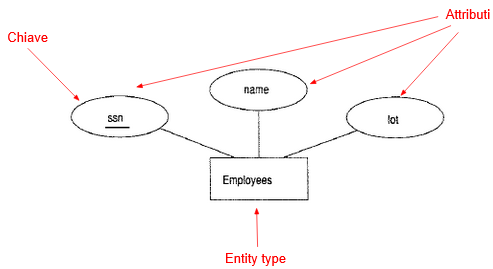
\includegraphics[width=0.5\textwidth]{04/ER-type.png}
                \caption{Rappresentazione di un \textit{entity type}}
            \end{figure}
    \subsection{Primo Raffinamento: le relazioni (\textit{relationships})}
        Si introducono dopo una prima fase di progettazione le relazioni. Una relazione (\textit{relationship}) è un'associazione tra due o più entità, come ad esempio l'associazione tra un dipendente e il suo dipartimento. Le relazioni dello stesso gruppo vengono raggruppate in un \textit{relationship set}. Il numero di \textit{entity type} che partecipano ad un \textit{relationship type} si dice \textbf{grado} della relazione.
        \paragraph{Attributi descrittivi}
            Una relazione può avere degli attributi che la descrivono, come ad esempio la data di inizio di un rapporto di lavoro tra un dipendente e un dipartimento. Gli attributi di una relazione forniscono solo informazioni su quella relazione, e \textbf{non} sulle entità che vi partecipano. Per questo motivo una relazione è identificata univocamente dalle entità che vi partecipano e \textbf{non} dagli attributi descrittivi.
        \paragraph{Relazioni ternarie} Come anticipato, una relazione può coinvolgere più di due \textit{entity type}, in tal caso si parla di relazione ternaria, quaternaria etc\dots In questo caso non avremo più solo due attributi che identificano la relazione, ma tre, quattro etc\dots Per il resto il concetto rimane invariato.
        \paragraph{Esempio} si consideri il seguente esempio di schema \texttt{ER}:
            \begin{figure}[H]
                \centering
                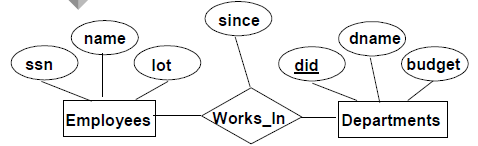
\includegraphics[width=0.5\textwidth]{04/ER-relations.png}
                \caption{Esempio di relazione tra due \textit{entity type}}
            \end{figure}
            Nell'esempio in figura la relazione "\texttt{Works\_In}" è di grado 2, in quanto coinvolge due \textit{entity type} (\texttt{Employees} e \texttt{Departments}).\newline
            Si noti come per una coppia degli attributi \texttt{<ssn, did>} si possa avere al massimo un solo valore per l'attributo \texttt{since} (ovvero la data di inizio del rapporto di lavoro tra un dipendente e un dipartimento).
        \paragraph{\textit{Relationship type} vs. \textit{relationship set}} Un \textit{relationship type} è lo schema che descrive la relazione, ne identifica il nome e gli \textit{entity types} che vi partecipano, infine identifica i vincoli associati ad essa. Un \textit{relationship set} è un insieme di istanze della relazione, rappresentate nella base di dati, con un parallelismo improprio e informale: "il \textit{relationship set} è lo stato attuale di un \textit{relationship type}".
    \subsection{Vincoli sulle relazioni}
        Distinguiamo in una relazione i seguenti vincoli:
        \begin{itemize}
            \item Vincoli di chiave (\textit{key constraints})
            \item Vincoli di cardinalità (\textit{cardinality ratio})
            \item Vincoli di esistenza o partecipazione (\textit{participation constraints})
        \end{itemize}
        \subsubsection{Vincoli di chiave}
            I vincoli di chiave permette di esprimere la condizione secondo la quale una entità possa partecipare al massimo una volta ad una relazione. Questo vincolo è espresso tramite una freccia con la punta annerita che parte dall'entità che può partecipare al massimo una volta e punta verso la relazione.
            \begin{figure}[H]
                \centering
                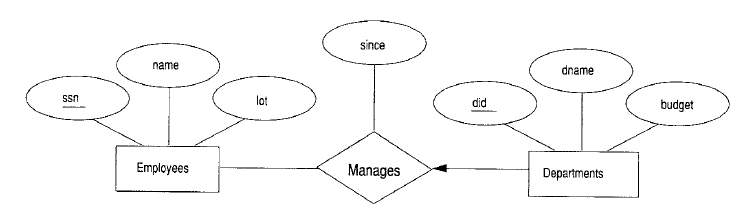
\includegraphics[width=0.5\textwidth]{04/ER-key-constraint.png}
                \caption{Vincolo di chiave}
            \end{figure}
            Nell'esempio: un dipartimento può avere al massimo un \textit{manager} (ovvero un dipendente), ma un dipendente può essere \textit{manager} anche di più dipartimenti.\newline
            Stessa cosa valer per le relazioni con grado maggiore di 2, per cui ad esempio un dipendente può lavorare su una sola sede di un dipartimento ma una sede può avere più dipendenti e un dipartimento può avere più sedi.
        \subsubsection{Vincoli di cardinalità}
            Servono a esprimere il numero \textbf{massimo} di volte che un'entità può \textbf{comparire} \footnote{Si noti che il vincolo di cardinalità non esprime il numero di volte che un'entità può partecipare ad una relazione, ma il numero di volte che un'entità può comparire in un \textit{relationship set}.} in un \textit{relationship set}. Questi vincoli sono espressi tramite una coppia di numeri, che indicano rispettivamente il numero minimo e massimo di volte che un'entità può comparire in un \textit{relationship set}.\newline
            Solitamente sono rappresentati ed espressi come:
            \begin{itemize}
                \item \textit{One-to-One} (1:1)
                \item \textit{One-to-Many} (1:N) o \textit{Many-to-One} (N:1)
                \item \textit{Many-to-One} (N:1)
            \end{itemize}
            Questi sono posti in prossimità della relazione, e sono separati da un trattino.
        \subsubsection{Vincoli di partecipazione}
            I vincoli di partecipazione specificano quante volte un'entità deve comparire \textbf{al minimo} in una relazione, per questi vincoli sono detti anche \textit{Existence Dependency Constraints}. 
            % TODO Finire la sotto-sotto-sezionle
\end{document}